\documentclass[12pt]{article}
\usepackage{amssymb,amsmath,graphicx,mathtools}
\usepackage{listings}
\usepackage[margin=0.75in]{geometry}
\parindent 16 pt
\usepackage{fancyhdr}
\pagestyle{fancy}
\fancyhead[R]{Swupnil Sahai}
\fancyhead[C]{11/30/16}
\fancyhead[L]{Kernel Model}
\DeclarePairedDelimiter\ceil{\lceil}{\rceil}
\DeclarePairedDelimiter\floor{\lfloor}{\rfloor}

\lstset{
    language=R,
    basicstyle=\scriptsize\ttfamily,
    stepnumber=1,
    numbersep=5pt,
    showspaces=false,
    showstringspaces=false,
    showtabs=false,
    frame=single,
    tabsize=2,
    captionpos=b,
    breaklines=true,
    breakatwhitespace=false,
    escapeinside={},
    keywordstyle={},
    morekeywords={}
    }

\begin{document}

% CUSTOM SHORTCUTS

\def\ci{\perp\!\!\!\perp}
\def\ex{\mathbb{E}}
\def\prob{\mathbb{P}}
\def\ind{\mathbb{I}}
\def\grad{\triangledown}
\def\bigo{\mathcal{O}}
\def\normal{\mathcal{N}}
\def\lognormal{\log\normal}

% INTRO %
\section{Introduction}
The class of models for aggregate relational data that we consider all involve modeling responses from a negative binomial distribution, with the mean $\mu_{ik}$ equal to the number of expected response for individual $i$ about knowing a number of people in a group of interest $\mathcal{G}_k$.

$$ y_{ik} \sim \text{NegBin}(\omega_k \mu_{ik}, \omega_k)
\hspace{20 pt} E(y_{ik}) = \mu_{ik} 
\hspace{20 pt} Var(y_{ik}) = \mu_{ik} + \frac{\mu_{ik}}{\omega_k}$$

% Random Mixing %
\subsection{Random Mixing}
\noindent The most basic model treats this expectation as simply $d_i$, the degree of individual $i$, multiplied by the proportion of the population that is in $\mathcal{G}_k$. Letting $\delta_{jk} = \ind\{ j \in \mathcal{G}_k\}$, we can derive this expression as follows:
\begin{align}
\mu_{ik} 
&= \sum_{j=1}^{d_i} \ex[ \delta_{jk} | i \to j ] && \\\nonumber
&= \sum_{j=1}^{d_i} \prob( j \in \mathcal{G}_k | i \to j ) && \\\nonumber
&= d_i \prob( j \in \mathcal{G}_k | i \to j ) && \\\nonumber
&= d_i \prob( j \in \mathcal{G}_k) && \\\nonumber
&= d_i \biggl( \frac{N_k}{N} \biggr)
\end{align}

% NON-RANDOM GENDER MIXING %
\subsection{Non-Random Gender Mixing}
If we do not want to simply assume that the way individual $i$ mixes with alters depends on gender then we can also model non-random gender mixing.
\begin{align}
\mu_{ik} 
&= \sum_{j=1}^{d_i} \prob( j \in \mathcal{G}_k | g_i, i \to j ) && \\\nonumber
&= d_i \prob( j \in \mathcal{G}_k | g_i, i \to j) && \\\nonumber
&= d_i \sum_{g_j} \prob( j \in \mathcal{G}_k, g_j | g_i, i \to j) && \\\nonumber
&= d_i \sum_{g_j} \prob( j \in \mathcal{G}_k | g_j, g_i, i \to j) p(g_j | g_i, i \to j) && \\\nonumber
&= d_i \sum_{g_j} \prob( j \in \mathcal{G}_k | g_j) \rho_{g_ig_j} && \\\nonumber
&= d_i \sum_{g_j} \rho_{g_ig_j} \prob( j \in \mathcal{G}_k | g_j)  && \\\nonumber
&= d_i \sum_{g_j} \rho_{g_ig_j} \biggl( \frac{N_{k,g_j}}{N_{g_j}} \biggr)
\end{align}

\noindent Here $\rho_{g_ig_j}$ is then a latent variable that can be inferred as the mixing rate between egos of gender $g_i$ and alters of gender $g_j$.

% NON-RANDOM AGE GENDER MIXING %
\subsection{Non-Random Age and Gender Mixing}
If we also believe that egos of certain ages might mix differently with alters of other ages, then, we can also model non-random age and gender mixing. Suppose the each individual $i$ belongs to some age category $a_i$ (e.g. 0-17, 18-24, etc.).
\begin{align}
\mu_{ik} 
&= \sum_{j=1}^{d_i} \prob( j \in \mathcal{G}_k | a_i, g_i, i \to j ) && \\\nonumber
&= d_i \prob( j \in \mathcal{G}_k | a_i, g_i, i \to j) && \\\nonumber
&= d_i \sum_{a_j,g_j} \prob( j \in \mathcal{G}_k, a_j, g_j | a_i, g_i, i \to j) && \\\nonumber
&= d_i \sum_{a_j,g_j} \prob( j \in \mathcal{G}_k | a_j, g_j, a_i, g_i, i \to j) p(a_j, g_j | a_i, g_i, i \to j) && \\\nonumber
&= d_i \sum_{a_j,g_j} \prob( j \in \mathcal{G}_k | a_j, g_j) \rho_{(a_i,g_i)(a_j,g_j)} && \\\nonumber
&= d_i \sum_{a_j,g_j} \rho_{(a_i,g_i)(a_j,g_j)} \prob( j \in \mathcal{G}_k | a_j, g_j)  && \\\nonumber
&= d_i \sum_{a_j,g_j} \rho_{(a_i,g_i)(a_j,g_j)} \biggl( \frac{N_{k,a_j,g_j}}{N_{a_j,g_j}} \biggr)
\end{align}

\noindent Here $\rho_{(a_i,g_i)(a_j,g_j)}$ is then a latent variable that can be inferred as the mixing rate between egos of age category $a_i$, gender $g_i$ and alters of age category $a_j$, gender $g_j$.

\subsection{Issues}
In our experiments, the non-random age-gender mixing model suffered from bias/variance and identifiability issues because the mixing rate parameters lacked constraints (other than summing to 1). In an effort to resolve this issue, we now propose a model with more structure and fewer parameters.

% MODEL %
\section{Kernel Model}
In this new approach, we first assume that age is continuous ($a_i \in (-\infty,\infty)$) rather than just binning age into categories. This allows us to model the mixing rate of an ego with age $a_i$ with an alter of age $a_j$ as a Gaussian kernel defined smoothly over all possible $a_j$.\\

\noindent Additionally, we also model the alter degree $d_j$ for the first time. Interestingly, this modeling yields different results depending on whether we set up the model from the perspective of the alter or from the perspective of the ego (as we've done in all previous models above). 

%% EGO PERSPECTIVE %%
\pagebreak
\subsection{Ego Perpsective}

\noindent Modifying the derivation from 1.3, the mean can be derived as follows:
\begin{align}
\mu_{ik} 
&= d_i \prob( j \in \mathcal{G}_k | a_i, g_i, i \to j) && \\\nonumber
&= d_i \sum_{g_j} \int_{a_j} \int_{d_j} \prob( j \in \mathcal{G}_k, a_j, g_j, d_j | a_i, g_i, i \to j) dd_j da_j && \\\nonumber
&= d_i \sum_{g_j} \int_{a_j} \int_{d_j} \prob( j \in \mathcal{G}_k | a_j, g_j, d_j, a_i, g_i, i \to j) p(a_j, g_j, d_j | a_i, g_i, i \to j) dd_j da_j && \\\nonumber
&= d_i \sum_{g_j} \int_{a_j} \int_{d_j} \prob( j \in \mathcal{G}_k | a_j, g_j) p(d_j | a_j, g_j, a_i, g_i, i \to j) 
p(a_j | g_j, a_i, g_i, i \to j) p(g_j | a_i, g_i, i \to j) dd_j da_j && \\\nonumber
&= d_i \sum_{g_j} \int_{a_j}  \prob( j \in \mathcal{G}_k | a_j, g_j) \biggl( \int_{d_j}  p(d_j | a_j, g_j, a_i, g_i, i \to j) dd_j \biggr)
p(a_j | g_j, a_i, g_i, i \to j) p(g_j | g_i, i \to j) da_j && \\\nonumber
&= d_i \sum_{g_j} \int_{a_j}  \prob( j \in \mathcal{G}_k | a_j, g_j) 
p(a_j | g_j, a_i, g_i, i \to j) p(g_j | g_i, i \to j) da_j && \\\nonumber
&= d_i \sum_{g_j} \int_{a_j} 
\biggl( \frac{ \sum_{a_j'} \prob( j \in \mathcal{G}_k | a_j', g_j) }{ \sum_{a_j'} \prob( j \in \mathcal{G}_k | a_j', g_j) } \biggr) 
\prob( j \in \mathcal{G}_k | a_j, g_j) p(a_j | a_i, g_i, g_j, i \to j) p(g_j | g_i, i \to j) da_j && \\\nonumber
&= d_i \sum_{g_j} p(g_j | g_i, i \to j) 
\biggl( \sum_{a_j'} \prob( j \in \mathcal{G}_k | a_j', g_j) \biggr) 
\int_{a_j} \biggl( \frac{ \prob( j \in \mathcal{G}_k | a_j, g_j) }{ \sum_{a_j'} \prob( j \in \mathcal{G}_k | a_j', g_j) } \biggr)
p(a_j | a_i, g_i, g_j, i \to j) da_j && \\\nonumber
&= d_i \sum_{g_j} \rho_{g_ig_j} 
\biggl( \sum_{a_j'} \prob( j \in \mathcal{G}_k | a_j', g_j) \biggr) 
\int_{a_j} \normal(a_j | \mu_{g_j,k}, \sigma_{g_j,k}^2)
\normal(a_j | a_i, \lambda_{g_ig_j}) da_j && \\\nonumber
&= d_i \sum_{g_j} \rho_{g_ig_j} 
\biggl( \sum_{a_j'} \frac{ N_{k, a_j', g_j} }{ N_{a_j', g_j} } \biggr) 
\frac{ e^{ -\frac{ (a_i - \mu_{g_j,k})^2 }{ 2(\lambda_{g_ig_j} + \sigma_{g_j,k}^2) } } }{ \sqrt{ 2\pi(\lambda_{g_ig_j} + \sigma_{g_j,k}^2) } }
\end{align}

\noindent Here $\rho_{g_ig_j}$ is the same latent variable as in 1.2 that can be inferred as the mixing rate between egos of gender $g_i$ and alters of gender $g_j$. Additionally, $\lambda_{g_ig_j}$ is a latent variable that can be inferred as the kernel bandwidth of the age mixing kernel. Essentially, small values of $\lambda_{g_ig_j}$ indicate that egos of gender $g_i$ only know alters of gender $g_j$ that are close to the ego in age (whereas larger values indicate the egos know alters of a wide range of ages, not necessarily just those close in age).\\

\noindent Additionally, $\mu_{g_j,k}$ and $\sigma_{g_j,k}^2$ are just estimated from the population data about group $G_k$. These values are analogous (though not exactly equal) to the mean and standard deviation of the ages of alters in group $G_k$ with gender $g_j$.

%% ALTER PERSPECTIVE %%
\pagebreak
\subsection{Alter Perspective}

\noindent  If we instead derive the same mean from the alter group's perspective, however, then we can derive the mean expression as follows:
\begin{align}
\mu_{ik}  &= \sum_{j \in \mathcal{G}_k} \ex[\delta_{ij} | a_i, g_i, d_i, j \in \mathcal{G}_k] 
&& \\\nonumber
&= N_k \prob(i \to j | a_i, g_i, d_i, j \in \mathcal{G}_k) 
&& \\\nonumber
&= N_k \sum_{g_j} \int_{a_j} \int_{d_j} \prob(i \to j | a_j, g_j, d_j, a_i, g_i, d_i, j \in \mathcal{G}_k) p(a_j, g_j, d_j | a_i, g_i, d_i, j \in \mathcal{G}_k) dd_j da_j 
&& \\\nonumber
&= N_k \sum_{g_j} \int_{a_j} \int_{d_j} \prob(i \to j | a_j, g_j, d_j, a_i, g_i, d_i) p(a_j, g_j, d_j | j \in \mathcal{G}_k) dd_j da_j 
&& \\\nonumber
&= N_k \sum_{g_j} \int_{a_j} \int_{d_j} \prob(i \to j | d_j, d_i, a_i, g_i) p(a_j, g_j | d_j, d_i, a_i, g_i, i \to j) p(d_j | a_j, g_j, j \in \mathcal{G}_k) p(a_j, g_j | j \in \mathcal{G}_k)  dd_j da_j 
&& \\\nonumber
&= N_k \sum_{g_j} \int_{a_j} \int_{d_j} \prob(i \to j | d_j, d_i) p(a_j, g_j | a_i, g_i, i \to j) p(d_j | a_j, g_j) p(a_j, g_j | j \in \mathcal{G}_k)  dd_j da_j 
&& \\\nonumber
&= N_k \sum_{g_j} \int_{a_j} \int_{d_j} \prob(i \to j | d_j, d_i) p(a_j | g_j, a_i, g_i, i \to j) p(g_j | a_i, g_i, i \to j) p(d_j | a_j, g_j) p(a_j, g_j | j \in \mathcal{G}_k)  dd_j da_j 
&& \\\nonumber
&= N_k \sum_{g_j} \int_{a_j} \int_{d_j} \biggl[ \frac{d_i d_j}{\sum_l d_l} \biggr]  p(a_j | g_j, a_i, g_i, i \to j) p(g_j|g_i, i \to j) p(d_j | a_j, g_j) p(a_j, g_j | j \in \mathcal{G}_k)  dd_j da_j 
&& \\\nonumber
&= N_k \sum_{g_j} p(g_j|g_i, i \to j) \int_{a_j} \int_{d_j}  \biggl[ \frac{d_i d_j}{N \bar{d}} \biggr]  p(a_j | g_j, a_i, g_i, i \to j) p(d_j | a_j, g_j) p(a_j | g_j, j \in \mathcal{G}_k) p(g_j | j \in \mathcal{G}_k) dd_j da_j 
&& \\\nonumber
&= d_i \frac{N_k}{N} \sum_{g_j} \rho_{g_ig_j} \int_{a_j} 
\biggl[ \frac{1}{\bar{d}} \int_{d_j} d_j p(d_j | a_j, g_j) dd_j \biggr] 
p(a_j | g_j, a_i, g_i, i \to j) p(a_j | g_j, j \in \mathcal{G}_k) p(g_j | j \in \mathcal{G}_k)  da_j 
&& \\\nonumber
&= d_i \frac{N_k}{N} \sum_{g_j} p(g_j | j \in \mathcal{G}_k) \rho_{g_ig_j} 
\int_{a_j} \frac{ \ex[d_j | a_j, g_j] }{ \bar{d} }  p(a_j | g_j, a_i, g_i, i \to j) p(a_j | g_j, j \in \mathcal{G}_k) da_j 
&& \\\nonumber
&= d_i \frac{N_k}{N} 
\sum_{g_j} \biggl( \frac{N_{k, g_j}}{N_k} \biggr) \rho_{g_ig_j} 
\int_{a_j} \ex\biggl[ \frac{d_j}{\bar{d}} \biggl| a_j, g_j \biggr]  \normal(a_j | a_i, \lambda_{g_ig_j}) \normal(a_j | \mu_{g_jk}, \sigma_{g_jk}^2) da_j 
&& \\\nonumber
&= d_i \sum_{g_j} \biggl( \frac{N_{k, g_j}}{N} \biggr)  \rho_{g_ig_j} 
\frac{ e^{ -\frac{(a_i - \mu_{g_jk})^2 } { 2(\lambda_{g_ig_j} + \sigma_{g_jk}^2) } } } { \sqrt{ 2\pi (\lambda_{g_ig_j} + \sigma_{g_jk}^2) } }  
\int_{a_j}  \ex\biggl[ \frac{d_j}{\bar{d}} \biggl| a_j, g_j \biggr] 
\normal \biggl(a_j \biggl| \frac{a_i \sigma_{g_jk}^2 + \mu_{g_jk} \lambda_{g_ig_j}}{\lambda_{g_ig_j} + \sigma_{g_jk}^2}, \frac{\lambda_{g_ig_j} \sigma_{g_jk}^2}{\lambda_{g_ig_j} + \sigma_{g_jk}^2} \biggr) da_j 
&& \\\nonumber
&= d_i \sum_{g_j} \rho_{g_ig_j} \biggl( \frac{N_{k, g_j}}{N} \biggr)
\frac{ e^{ -\frac{(a_i - \mu_{g_jk})^2 } { 2(\lambda_{g_ig_j} + \sigma_{g_jk}^2) } } } { \sqrt{ 2\pi (\lambda_{g_ig_j} + \sigma_{g_jk}^2) } }  
\ex\biggl[ \frac{d_j}{\bar{d}} \biggl| g_j \biggr] 
\end{align}

\noindent We now derive $\ex\biggl[ \frac{d_j}{\bar{d}} \biggl| g_j \biggr]$ on the next page.

%% CONTINUOUS AGE NON CONSTANT DEGREE %%
\pagebreak
\subsubsection{Non-Constant Alter Degree}

\noindent  If we assume that an individual's degree $d_j$ follows a log normal distribution $ d_j \sim \lognormal(\beta_1 + \beta_2 g_j - \beta_3 (a_j - \bar{a})^2, \eta^2)$ with $\beta_3 > 0 $, then we can derive $\ex\biggl[ \frac{d_j}{\bar{d}} \biggl| g_j \biggr]$ as follows:

\begin{align}
\ex\biggl[ \frac{d_j}{\bar{d}} \biggl| g_j \biggr] 
&= \int_{a_j}  \ex\biggl[ \frac{d_j}{\bar{d}} \biggl| a_j, g_j \biggr] 
\normal \biggl(a_j \biggl| \frac{a_i \sigma_{g_jk}^2 + \mu_{g_jk} \lambda_{g_ig_j}}{\lambda_{g_ig_j} + \sigma_{g_jk}^2}, \frac{\lambda_{g_ig_j} \sigma_{g_jk}^2}{\lambda_{g_ig_j} + \sigma_{g_jk}^2} \biggr) da_j 
&& \\\nonumber
&= \int_{a_j} e^{ \beta_1 + \beta_2 g_j - \beta_3 (a_j - \bar{a})^2 + \frac{\eta^2}{2} } 
\normal \biggl(a_j \biggl| \frac{a_i \sigma_{g_jk}^2 + \mu_{g_jk} \lambda_{g_ig_j}}{\lambda_{g_ig_j} + \sigma_{g_jk}^2}, \frac{\lambda_{g_ig_j} \sigma_{g_jk}^2}{\lambda_{g_ig_j} + \sigma_{g_jk}^2} \biggr) da_j
 && \\\nonumber
&= \frac{ e^{ \beta_0 + \beta_2 g_j + \frac{\eta^2}{2} } }{ \bar{d} }
\int_{a_j} e^{- \beta_3 (a_j - \bar{a})^2} 
\normal \biggl(a_j \biggl| \frac{a_i \sigma_{g_jk}^2 + \mu_{g_jk} \lambda_{g_ig_j}}{\lambda_{g_ig_j} + \sigma_{g_jk}^2}, \frac{\lambda_{g_ig_j} \sigma_{g_jk}^2}{\lambda_{g_ig_j} + \sigma_{g_jk}^2} \biggr) da_j 
&& \\\nonumber
&= \frac{ e^{ \beta_0 + \beta_2 g_j + \frac{\eta^2}{2} } }{ \bar{d} }
\int_{a_j} \frac{ 1 }{ \sqrt{ \frac{\beta_3}{\pi} } }
\frac{ e^{- \frac{ (a_j - \bar{a})^2 }{ 2 ( \frac{1}{2\beta_3} ) } } }{ \sqrt{ 2 \pi (\frac{1}{2\beta_3}) } }
\normal \biggl(a_j \biggl| \frac{a_i \sigma_{g_jk}^2 + \mu_{g_jk} \lambda_{g_ig_j}}{\lambda_{g_ig_j} + \sigma_{g_jk}^2}, \frac{\lambda_{g_ig_j} \sigma_{g_jk}^2}{\lambda_{g_ig_j} + \sigma_{g_jk}^2} \biggr) da_j 
&& \\\nonumber
&= \frac{ e^{ \beta_0 + \beta_2 g_j + \frac{\eta^2}{2} } }{ \bar{d} \sqrt{ \frac{\beta_3}{\pi} } }
\int_{a_j} \normal \biggl(a_j \biggl| \bar{a}, \frac{1}{2\beta_3} \biggr)
\normal \biggl(a_j \biggl| \frac{a_i \sigma_{g_jk}^2 + \mu_{g_jk} \lambda_{g_ig_j}}{\lambda_{g_ig_j} + \sigma_{g_jk}^2}, \frac{\lambda_{g_ig_j} \sigma_{g_jk}^2}{\lambda_{g_ig_j} + \sigma_{g_jk}^2} \biggr) da_j 
&& \\\nonumber
&= \frac{ e^{ \beta_0 + \beta_2 g_j + \frac{\eta^2}{2} } }{ \bar{d} \sqrt{ \frac{\beta_3}{\pi} } }
\frac{1}{ \sqrt{ 2 \pi ( \frac{1}{2\beta_3} + \frac{\lambda_{g_ig_j} \sigma_{g_jk}^2}{\lambda_{g_ig_j} + \sigma_{g_jk}^2} ) } }
\exp\biggl\{ -\frac{ ( \bar{a} - \frac{a_i \sigma_{g_jk}^2 + \mu_{g_jk} \lambda_{g_ig_j}}{\lambda_{g_ig_j} + \sigma_{g_jk}^2} )^2 }{ 2 ( \frac{1}{2\beta_3} + \frac{\lambda_{g_ig_j} \sigma_{g_jk}^2}{\lambda_{g_ig_j} + \sigma_{g_jk}^2} ) } \biggr\}
&& \\\nonumber
&\hspace{10 pt}\cdot \int_{a_j} \normal \biggl(a_j \biggl| 
\frac{ ( \bar{a} )\frac{\lambda_{g_ig_j} \sigma_{g_jk}^2}{\lambda_{g_ig_j} + \sigma_{g_jk}^2} 
+ \biggl( \frac{a_i \sigma_{g_jk}^2 + \mu_{g_jk} \lambda_{g_ig_j}}{\lambda_{g_ig_j} + \sigma_{g_jk}^2} \biggr) \frac{1}{2\beta_3} }
{ \frac{1}{2\beta_3} + \frac{\lambda_{g_ig_j} \sigma_{g_jk}^2}{\lambda_{g_ig_j} + \sigma_{g_jk}^2} }, 
\frac{ \frac{1}{2\beta_3}\frac{\lambda_{g_ig_j} \sigma_{g_jk}^2}{\lambda_{g_ig_j} + \sigma_{g_jk}^2} }{ \frac{1}{2\beta_3} + \frac{\lambda_{g_ig_j} \sigma_{g_jk}^2}{\lambda_{g_ig_j} + \sigma_{g_jk}^2} } \biggr) da_j
&& \\\nonumber
&= \frac{ e^{ \beta_0 + \beta_2 g_j + \frac{\eta^2}{2} } }{ \bar{d} \sqrt{ 2 \pi ( \frac{1}{2\beta_3} + \frac{\lambda_{g_ig_j} \sigma_{g_jk}^2}{\lambda_{g_ig_j} + \sigma_{g_jk}^2} ) }  }
\exp\biggl\{ -\frac{ ( \bar{a} - \frac{a_i \sigma_{g_jk}^2 + \mu_{g_jk} \lambda_{g_ig_j}}{\lambda_{g_ig_j} + \sigma_{g_jk}^2} )^2 }{ 2 ( \frac{1}{2\beta_3} + \frac{\lambda_{g_ig_j} \sigma_{g_jk}^2}{\lambda_{g_ig_j} + \sigma_{g_jk}^2} ) } \biggr\}
\end{align}

%% CONTINUOUS AGE CONSTANT DEGREE %%
\subsubsection{Constant Degree}
\noindent  If we instead assume that $d_j = \bar{d}$ for all alters, then we can simplify $\ex\biggl[ \frac{d_j}{\bar{d}} \biggl| g_j \biggr]$ as follows:

\begin{align}
\ex\biggl[ \frac{d_j}{\bar{d}} \biggl| g_j \biggr] 
&= \int_{a_j} \ex\biggl[ \frac{d_j}{\bar{d}} \biggl| a_j, g_j \biggr] 
\normal \biggl(a_j \biggl| \frac{a_i \sigma_{g_jk}^2 + \mu_{g_jk} \lambda_{g_ig_j}}{\lambda_{g_ig_j} + \sigma_{g_jk}^2}, \frac{\lambda_{g_ig_j} \sigma_{g_jk}^2}{\lambda_{g_ig_j} + \sigma_{g_jk}^2} \biggr) da_j 
&& \\\nonumber
&= \int_{a_j} \ex\biggl[ \frac{\bar{d}}{\bar{d}} \biggl| a_j, g_j \biggr] 
\normal \biggl(a_j \biggl| \frac{a_i \sigma_{g_jk}^2 + \mu_{g_jk} \lambda_{g_ig_j}}{\lambda_{g_ig_j} + \sigma_{g_jk}^2}, \frac{\lambda_{g_ig_j} \sigma_{g_jk}^2}{\lambda_{g_ig_j} + \sigma_{g_jk}^2} \biggr) da_j 
&& \\\nonumber
&= \int_{a_j}  
\normal \biggl(a_j \biggl| \frac{a_i \sigma_{g_jk}^2 + \mu_{g_jk} \lambda_{g_ig_j}}{\lambda_{g_ig_j} + \sigma_{g_jk}^2}, \frac{\lambda_{g_ig_j} \sigma_{g_jk}^2}{\lambda_{g_ig_j} + \sigma_{g_jk}^2} \biggr) da_j 
&& \\\nonumber
&= 1
\end{align}

%SIMULATION%
\section{Simulation}
\subsection{Data}
We simulate responses to questions about 12 names using estimated age means/variances (for each name), degree regression coefficients, simulated respondent degrees, name overdispersions, kernel lengthscales, and gender mixing rates in an attempt to determine whether our model can recover the parameters. 

$$
\beta = [6.256, -0.005, -6.908] 
\hspace{20 pt}
\eta = 0.5 
\hspace{20 pt}
d_j \sim \lognormal(\beta_1 + \beta_2 g_j - e^{\beta_3} (a_j - \bar{a})^2, \eta^2)
$$

\noindent \begin{tabular}{c | cccccccccccc} 
Var & Linda & Jen. & Karen & Kim. & Emily & Steph. & Mark & Jacob & Kevin & Kyle & Adam & Bruce \\
\hline
$\mu_k$ & 63.3 & 37.4 & 56.1 & 39.8 & 28.0 & 35.6 & 49.2 & 22.5 & 38.8  & 25.6 & 31.0 & 62.4 \\
$\sigma_k$ & 10.4 & 10.6 & 13.9 & 13.0 & 22.9 & 14.3 & 14.9 & 18.0 & 16.2 & 10.8 & 16.2 & 16.7  \\
$\omega_k$ & 4.23 & 8.42 & 7.65 & 3.83 & 9.79 & 10.91 & 5.01 & 2.80 & 2.22 & 2.60 & 12.69 & 4.95  \\
\end{tabular}\\

$$ \lambda
= \left( \begin{array}{cc} \lambda_{FF} & \lambda_{FM} \\
\lambda_{MF} & \lambda_{MM} \end{array} \right) 
= \left( \begin{array}{cc}
225 & 144 \\
100 & 256 \end{array} \right)
\hspace{20 pt}
\rho
= \left( \begin{array}{cc} \rho_{FF} & \rho_{FM} \\
\rho_{MF} & \rho_{MM} \end{array} \right) 
= \left( \begin{array}{cc}
0.6 & 0.4 \\
0.45 & 0.55 \end{array} \right) $$ \vspace{7 pt}

%PRIORS%
\subsection{Priors}
\noindent The following priors were used:

$$
\beta \sim \normal(0, 2I)
\hspace{15 pt}
\eta \sim \lognormal(-0.7, 0.1)
\hspace{15 pt}
d_j \sim \lognormal(\beta_1 + \beta_2 g_j - e^{\beta_3} (a_j - \bar{a})^2, \eta^2)
$$
$$
\rho_{g_i\cdot} \sim Alpha(5,5)
\hspace{15 pt}
\lambda_{g_ig_j} \sim \lognormal(\log 100, 0.5)
\hspace{15 pt}
\frac{1}{ \frac{1}{\omega_k}+1} \sim Beta(4.5,0.5)
$$

%RESULTS%
% DEGREE
\pagebreak
\subsection{Results}
\subsubsection*{Respondent Degrees ($d_i$)}
\noindent The degrees are recovered well.

\begin{center}
\includegraphics[scale = 0.34]{Estimates_Degree_Regression.png}
\end{center}

% LAMBDA
\subsubsection*{Kernel Lengthscale ($\lambda_{g_ig_j}$)}
The continuous model does a decent job of recovering the kernel lengthscales.

\begin{center}
\includegraphics[scale = 0.34]{Estimates_Lambda_Regression.png}
\end{center}

%MIXING%
\pagebreak
\subsubsection*{Gender Mixing Rates ($\rho_{g_ig_k}$)}
\noindent the gender mixing rates are recovered decently well.

\begin{center}
\includegraphics[scale = 0.34]{Estimates_Mixing_Regression.png}
\end{center}

%BETA%
\subsubsection*{Degree Regression Parameters ($\beta_j$)}
\noindent Lastly, the beta regression parameters are recovered very well.

\begin{center}
\includegraphics[scale = 0.34]{Estimates_Beta_Regression.png}
\end{center}

% OMNI DATA %
\pagebreak
\section{Omni Data Results}
\subsubsection*{Respondent Degrees}
The continuous model estimates imply decreasing and then increasing network size by age for men, but monotonically decreasing network size by age for women.

\begin{center}
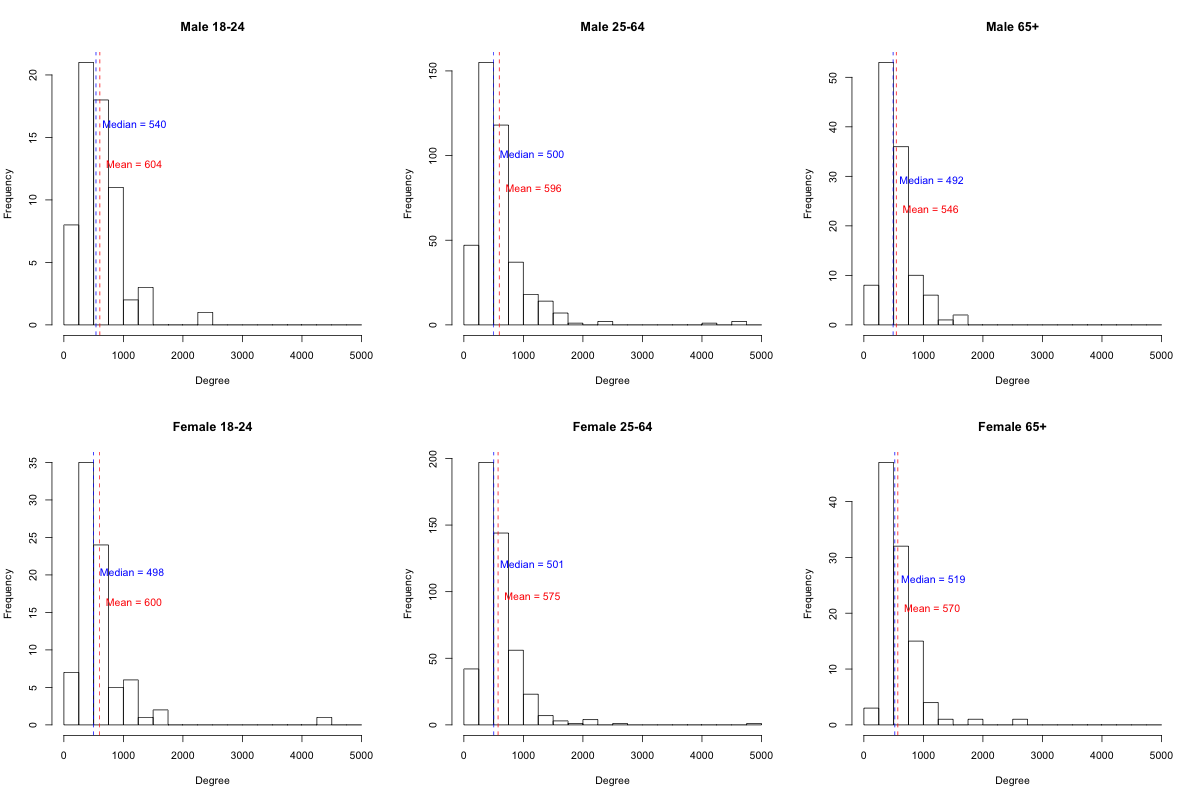
\includegraphics[scale = 0.36]{Estimates_Degree_Omni.png}
\end{center}

\subsubsection*{Gender Mixing Rates}
\noindent The gender mixing rates imply male-dominated networks. In general, about 56\% of a female's network is female, while 59\% of a male's network is male. This also implies that females mix more with males than the other way around.

$$ \rho_{BAYES}
= \left( \begin{array}{cc} \rho_{FF} & \rho_{FM} \\
\rho_{MF} & \rho_{MM} \end{array} \right) 
= \left( \begin{array}{cc}
0.44 & 0.56 \\
0.41 & 0.59 \end{array} \right) $$

% KERNEL LENTGHSCALES
\pagebreak
\subsubsection*{Kernel Lengthscales}
\noindent The length scales estimated from the actual data are large, implying very flat kernels. The important distinction here, then, is perhaps the relative size of the lengthscales.

$$ \lambda_{BAYES}
= \left( \begin{array}{cc} \lambda_{FF} & \lambda_{FM} \\
\lambda_{MF} & \lambda_{MM} \end{array} \right) 
= \left( \begin{array}{cc}
969 & 1253 \\
1104 & 1153 \end{array} \right) $$ \vspace{7 pt}

\noindent Indeed, it seems that the female to female kernel is much tighter than the male to male kernel, implying that women tend to know a narrow age range of other women but men tend to know a wide age range of other men. Alternatively, the female to male kernel is much wider than the male to female kernel, implying that women know a wider age range of men while men known a relatively narrow age range of women.

\begin{center}
\includegraphics[scale = 0.36]{Estimates_Kernel_Omni.png}
\end{center}

% MCCARTY DATA %
\pagebreak
\section{McCarty Data Results}
\subsubsection*{Respondent Degrees}
The continuous model estimates imply decreasing and then increasing network size by age for men, but monotonically decreasing network size by age for women.

\begin{center}
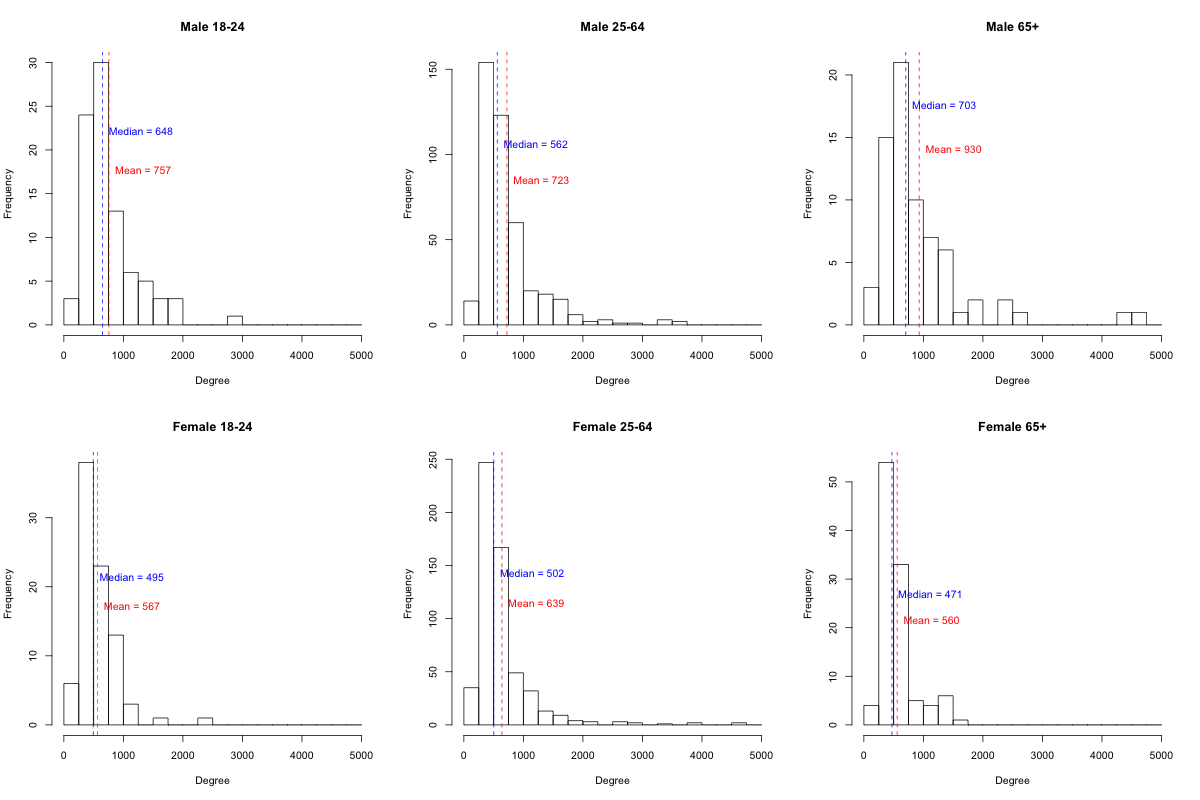
\includegraphics[scale = 0.36]{Estimates_Degree_McCarty.png}
\end{center}

\subsubsection*{Gender Mixing Rates}
\noindent The gender mixing rates imply male-dominated networks. In general, about 69\% of a female's network is female, while 64\% of a male's network is male. This also implies that females mix more with males than the other way around.

$$ \rho_{BAYES}
= \left( \begin{array}{cc} \rho_{FF} & \rho_{FM} \\
\rho_{MF} & \rho_{MM} \end{array} \right) 
= \left( \begin{array}{cc}
0.31 & 0.69 \\
0.36 & 0.64 \end{array} \right) $$

% KERNEL LENTGHSCALES
\pagebreak
\subsubsection*{Kernel Lengthscales}
\noindent The length scales estimated from the actual data are large, implying very flat kernels. The important distinction here, then, is perhaps the relative size of the lengthscales.

$$ \lambda_{BAYES}
= \left( \begin{array}{cc} \lambda_{FF} & \lambda_{FM} \\
\lambda_{MF} & \lambda_{MM} \end{array} \right) 
= \left( \begin{array}{cc}
1237 & 1255 \\
698 & 835 \end{array} \right) $$ \vspace{7 pt}

\noindent Indeed, it seems that the female to female kernel isn't as tight as the male to male kernel, implying that women tend to know a wide age range of other women but men tend to know a narrow age range of other men. Alternatively, the female to male kernel is much wider than the male to female kernel, implying that women know a wider age range of men while men known a relatively narrow age range of women.

\begin{center}
\includegraphics[scale = 0.36]{Estimates_Kernel_McCarty.png}
\end{center}

\end{document}